\documentclass[11pt]{article}
\usepackage[margin=1in]{geometry}
\usepackage[T1]{fontenc}
\usepackage{lmodern,amsmath,amssymb,amsthm,booktabs,graphicx,microtype}
\usepackage[numbers,sort&compress]{natbib}
\usepackage{xcolor}
\usepackage[colorlinks=true,linkcolor=blue!55!black,citecolor=blue!55!black,%
            urlcolor=blue!55!black]{hyperref}
\hypersetup{%
  pdftitle={Exposure and amplitude limits for eradicating populations with inherited cellular states},
  pdfsubject={Feedback exposure bounds, amplitude floors, and certified molecular branching examples}}
\usepackage{enumitem}
\setlist{nosep}

\renewcommand{\topfraction}{.9}\renewcommand{\bottomfraction}{.6}
\renewcommand{\textfraction}{.08}\renewcommand{\floatpagefraction}{.8}

\newtheorem{theorem}{Theorem}[section]
\newtheorem{lemma}[theorem]{Lemma}
\newtheorem{corollary}[theorem]{Corollary}
\newtheorem{proposition}[theorem]{Proposition}
\theoremstyle{remark}\newtheorem{remark}[theorem]{Remark}

\newcommand{\E}{\mathbb E}\newcommand{\Prob}{\mathbb P}
\newcommand{\one}{\mathbf1}\newcommand{\PhiB}{\Phi_{\mathrm{base}}}
\newcommand{\R}{\mathbb R}\newcommand{\N}{\mathbb N}
\DeclareMathOperator{\diag}{diag}
\DeclareMathOperator{\spb}{s}

\title{Exposure and amplitude limits for eradicating populations\\
with inherited cellular states}
\author{}
\date{20 September 2026}

\begin{document}
\maketitle

\begin{abstract}
How much intervention is necessary to eradicate a finite population whose cells
inherit a molecular state, when the intervention may be chosen using the entire
population history? We prove two independent obstructions for finite-type
branching populations under bounded predictable feedback. The first is an
exposure floor: a baseline extinction supersolution together with a
componentwise bound on the intervention generator produces a family of
supersolutions indexed by the remaining budget, and the resulting population
barrier retains founder-count dependence without assuming that families are
independent under feedback; for $n$ identical founders it gives survival
probability at least $1-(1-\eta e^{-cB})^n$. The second is an amplitude floor:
a single supersolution valid across the whole admitted action range bounds
survival away from zero for \emph{every} policy, at every budget and every
horizon. Necessary and sufficient exposures match at order $\log(n/\delta)$
above the amplitude threshold, and an outward-rounded Taylor calculation
certifies a finite-time policy at exposure $11.6$ with risk below $0.01$ from
one founder of the two-site molecular source. We then locate the amplitude
threshold exactly in that source as a function of memory size: the critical
intrinsic erasure is bracketed to six decimals for $2\le N\le 8$ sites and rises
from $.0927$ to $.4506$, so at five to eight sites no policy of amplitude $.29$
eradicates, whatever its budget or duration; explicit rational supersolutions
bound the surviving probability below by $.17$, $.46$, $.61$ and $.70$ at
$N=5,\dots,8$. A second actuator repairs this: added death on protected states
has an $N$-uniform threshold $b-d_{\mathrm{prot}}$, gives a dimension-free
sufficient exposure $1.45\log(n/\delta)$, and attains the exposure floor up to a
factor below $1.54$. We also record a preparation-dependent failure of
monotonicity in erasure, and conditional concentration and administered-amount
lower bounds. Probability proofs are conventional; source certificates and the
finite-time enclosure are exact finite computations; selected algebra is
checked in Lean.
\end{abstract}

\tableofcontents

\section{Introduction}
\label{sec:intro}

An inherited state can affect both the descendants a cell produces and their
susceptibility to killing. Eliminating a marker along one lineage therefore
need not eliminate the family. Conversely, a declining expected population can
give a useful extinction guarantee, but a negative mean growth rate alone does
not quantify finite-founder survival. The appropriate control question concerns
the probability of leaving any surviving family under an explicitly priced
intervention.

Reaction-based models connect histone and DNA modifications to cellular memory
\citep{dodd2007,bruno,bruno2024}, and inherited non-genetic states are a
standard explanation for drug-tolerant persistence
\citep{balaban2004,sharma2010,shaffer2017,oren2021}. Inheritance and treatment
resistance have been studied in population models \citep{cassidy}; drug-induced
plasticity changes optimal dosing, and the chosen dose--response law can change
which schedules are favored \citep{gunnarsson}. Controlled branching processes
have a substantial stochastic-control theory \citep{claisse,kimmel2015}, and
tumour elimination probabilities have been used directly in treatment
objectives \citep{burroughs}. We do not claim priority for branching generating
functions, stochastic verification, or extinction-based treatment objectives.
Our contribution is a pair of explicit, checkable certificates --- one indexed
by the remaining budget, one uniform over the admitted action range --- their
founder-count and memory-size consequences, and a source-level realization that
retains correlated molecular inheritance.

\subsection*{Two obstructions, and a third}

Write $B$ for the total intervention exposure, meaning additional molecular
reaction rate integrated over time, and $v_{\max}$ for the largest instantaneous
rate the actuator can deliver. Three separate quantities can prevent
eradication.

\begin{itemize}
\item \textbf{Exposure.} Theorem~\ref{thm:main} shows that if a baseline
extinction supersolution $q$ obeys a componentwise inequality $Rq\le c(1-q)$
for the intervention generator, then survival from configuration $z$ is at
least $1-\prod_i[1-e^{-cB}(1-q_i)]^{z_i}$ for \emph{every} predictable policy
respecting the pathwise budget $B$. The exposure needed to reach risk $\delta$
from $n$ founders therefore grows like $c^{-1}\log(n/\delta)$.
\item \textbf{Amplitude.} Theorem~\ref{thm:amp} shows that if a single $q$ is a
supersolution for every admitted action --- equivalently, by affineness, at
both ends of the action range --- then survival is at least $1-\prod_iq_i^{z_i}$
for every policy at \emph{every} budget and horizon. This obstruction is not
removed by treating longer or paying more.
\item \textbf{Time.} Proposition~\ref{prop:time} shows that bounded death rates
impose a minimum duration for finite-time extinction, independently of the two
bounds above.
\end{itemize}

The three are logically independent, and they fail in different ways. Only the
first is a budget statement; only the second survives an unbounded course; only
the third constrains a fixed deadline.

\subsection*{What is new relative to the exposure floor alone}

The central technical device for the exposure floor is that no optimization over
a discretized population space is required. Given a baseline supersolution $q$,
one considers the entire segment $1-a(1-q)$, which is preserved by the
inequality a population barrier needs (Lemma~\ref{lem:segment}); setting $a$ by
the remaining budget gives a bound that approaches one with founder count at
every fixed finite exposure. A constant admissible action with a negative
weighted drift gives the matching logarithmic order
(Corollary~\ref{cor:order}), and an outward-rounded Taylor enclosure certifies a
sharper finite-horizon policy in the worked source
(Section~\ref{sec:pulse}).

The amplitude floor is what makes the memory-size question answerable. In the
molecular source of Section~\ref{sec:source} the erasure actuator has a
critical amplitude $v_c(N)$: below it the certificates exhibited here show that
\emph{no} policy eradicates, and above it a constant action does.
Section~\ref{sec:memory} brackets the corresponding
critical intrinsic erasure to six decimals for $2\le N\le8$ sites; it rises from
$.092750$ at two sites to $.450572$ at eight, a factor of $4.86$. In particular
the amplitude $.29$ used in the two-site worked example is certified
\emph{insufficient at any budget or duration} for $5\le N\le8$, with explicit
rational supersolutions bounding survival from a fully marked founder below by
$.170$, $.460$, $.613$ and $.701$ at $N=5,6,7,8$. This settles, negatively, a
question left open by a coarser mean-growth diagnostic, which had only shown
that a particular constant action ceases to contract.

Section~\ref{sec:memory} also shows that the deterioration is a property of this
actuator and not of inherited memory as such. A second actuator that adds death
on protected states has threshold at most $b-d_{\mathrm{prot}}$ for every $N$,
because beyond that value the expected total count decays at rate
$\min(\kappa-(b-d_{\mathrm{prot}}),\,d_{\mathrm{unprot}}-b)$ with unit weight
vector; the resulting sufficient exposure $1.45\log(n/\delta)$ is dimension-free
and lies within a factor $1.54$ of the exposure floor at $n=1$, $\delta=.01$.
Where the eraser alone needs a fourfold amplitude increase between two and eight
sites, a fixed added death of $.025$ restores mean contraction at six sites at
the erasure amplitude that by itself provably fails.

\subsection*{Scope}

The case study uses synthetic reaction and demographic rates. It is suitable for
exposing mathematical dependencies and for designing a low-density microcolony
test, not for prescribing a drug regimen. The exposure variable measures
additional molecular reaction rate integrated over time; it is not a drug mass
or a concentration, and Section~\ref{sec:pkpd} states exactly what is needed to
convert it. Throughout, ``eradication'' means the specified extinction event in
a process with no immigration, and ``survival'' means non-extinction of the
mathematical population, which is not a detection threshold, a clinical
recurrence or a progression endpoint.

\section{Controlled inherited-state populations}
\label{sec:model}

Let $\{1,\ldots,m\}$ be a finite type space and $Z_t\in\N^m$ the count vector.
A cell of type $i$ changes type according to a conservative generator $Q$,
dies at rate $d_i$, and is replaced at rate $b_i$ by an offspring vector with
probability generating function $F_i(x)$. Offspring types may be correlated; the
joint offspring law is part of the data. We assume a deterministic upper bound
$K$ on offspring count, and that all per-cell rates are bounded over the
admitted action set. Define
\begin{equation}\label{eq:field}
 \Phi(x)=Qx+d\odot(1-x)+b\odot(F(x)-x),
\end{equation}
where $\odot$ is the entrywise product. For binary offspring write
$F_i(x)=D_i(x,x)$ with $D_i$ the bilinear form of the ordered daughter law; the
mother's removal accounts for the term $-b_ix_i$.

Under deterministic rates, conditional independence of future offspring clocks
given their birth states gives the backward equation $\dot u=\Phi(u)$. With
terminal datum zero its solution is extinction by the horizon. A terminal datum
$q^{\mathrm{off}}$ instead represents eventual extinction under a specified
continuation after the course. For piecewise constant schedules the autonomous
flows act on this terminal datum in reverse chronological order.

\subsection{Actions, feedback and budget}

During intervention use $Q_v=Q_{\mathrm{base}}+vR$ with $R\one=0$ and
$0\le v_t\le v_{\max}$, each $Q_v$ a valid generator. We write $\PhiB$ for
\eqref{eq:field} at $v=0$ and $\Phi_v$ for the field with $Q_v$ in place of $Q$.
The scalar common action is predictable with respect to the entire population
history and any independent controller randomization. It obeys the pathwise
constraint
\begin{equation}\label{eq:budget}
 C_t=\int_0^tv_s\,ds\le B \qquad(0\le t\le T)
 \qquad\text{almost surely.}
\end{equation}
The constraint is pathwise, not an expectation constraint: replacing
\eqref{eq:budget} by $\E C_T\le B$ requires a different argument. Nor is $B$ a
sum of cell-specific exposures; the common-control budget is a single number
spent by a single actuator. The background death and reproduction rates are
fixed unless an extension explicitly changes them. This full-information
feedback class contains any controller using less information. Families need not
be independent under it.

The process is constructed by predictable thinning of bounded Poisson proposals
on a countable genealogical tree. Birth count is dominated by a
bounded-offspring pure-birth process, with expected size at most
$|Z_0|e^{b_{\max}(K-1)t}$ for $K\ge1$. Expected proposal counts on finite
intervals are finite, which proves non-explosion by localization. Empty
populations remain empty, so $0$ is absorbing and there is no immigration.
Feedback changes conditional intensities; it does not invalidate this
construction. A \emph{continuation} is a specified uncontrolled branching
source, started with fresh randomness conditional on the population at
withdrawal.

\subsection{The population generator identity}

For $x\in(0,1]^m$ put $V_x(z)=\prod_ix_i^{z_i}$. A type change, a death and a
reproduction multiply $V_x$ by $x_j/x_i$, by $1/x_i$ and by the offspring
monomial divided by $x_i$, respectively. Summing conditional rates, the actual
population generator obeys
\begin{equation}\label{eq:generator}
 \mathcal G_vV_x(z)=V_x(z)\sum_iz_i\frac{\Phi_v(x)_i}{x_i}.
\end{equation}
This is an identity on the population state space. It remains valid under
feedback because it is conditional on the current predictable action, and it
makes no assertion that cells exposed to a common controller have independent
histories; it does not factor founder probabilities. Conditional independence
is used later only for a fixed baseline continuation, once the population at
withdrawal is given.

\subsection{First moments}
\label{sec:firstmoment}

Write $L$ for the expected offspring matrix, $L_{ij}=\E[\#\{\text{daughters of
type }j\}\mid\text{mother of type }i]$, so that $L=2\Lambda$ for binary division
with single-daughter marginal $\Lambda$. The first-moment matrix at constant
action $v$ is
\begin{equation}\label{eq:meanmatrix}
 A_v=Q_v+\diag(b)\,(L-I)-\diag(d),
\end{equation}
acting on weight vectors from the left index, so that $W(z)=\sum_iz_iw_i$ has
drift $\sum_iz_i(A_vw)_i$. Equivalently, $A_v$ is the linearization of $\Phi_v$
at $x=\one$ up to sign: $D\Phi_v(\one)=-A_v$. It is a Metzler matrix. The
one-daughter marginal determines $A_v$ but not the extinction probabilities;
sibling correlation lives in the joint law $D$ and is retained throughout.

\subsection{Endpoints that must stay distinct}
\label{sec:endpoints}

Write
\[
 s_\pi(T)=\Prob_\pi(|Z_T|>0),\qquad
 r_\pi(T)=\Prob_\pi(\text{non-extinction under the specified continuation
 after }T).
\]
Then $s_\pi(T)\ge r_\pi(T)$, because extinction is absorbing and the
continuation has no immigration. A finite-time survival \emph{upper} bound
therefore also bounds eventual survival; a lower bound on eventual survival also
lower-bounds finite-time survival, provided its continuation assumptions hold.
Our principal continuation withdraws the additional eraser, restoring baseline
erasure while retaining the background demographic rates. Withdrawing the
background killing as well is a different experiment, and
Section~\ref{sec:withdrawal} keeps the two separate.

\subsection{Units}
\label{sec:units}

Reaction, division and death rates have units of inverse time. The integrated
exposure $B=\int v\,dt$ is dimensionless when $v$ is an additional first-order
rate. Neither $B$ nor $v$ is a drug mass or a concentration. A
nondimensionalization choosing a reference division rate $b_0$, setting
$\hat t=b_0t$ and dividing all rates by $b_0$ leaves $\int v\,dt$ unchanged, so
exposure statements transfer between time units; changing the clock alone does
not calibrate the relative biology. For the synthetic source of
Section~\ref{sec:source}, $b_0=.1$ and time $100$ spans ten mean division
waiting times.

\section{The remaining-exposure theorem}
\label{sec:exposure}

\begin{lemma}[Supersolution segment]\label{lem:segment}
Suppose $q\in(0,1]^m$, $\PhiB(q)\le0$, and let $h=1-q$. For $0\le a\le1$,
$q_a=1-ah$ satisfies $\PhiB(q_a)\le0$. In the binary case, exactly
\begin{equation}\label{eq:segment}
 \PhiB(1-ah)=a\PhiB(q)-a(1-a)\,b\odot D(h,h).
\end{equation}
If $Rq\le ch$ for $c\ge0$, then $Rq_a\le c(1-q_a)$.
\end{lemma}

\begin{proof}
Conservation of $Q$ and normalization $F(1)=1$ give $\PhiB(1)=0$. For binary
offspring, expand $D(1-ah,1-ah)$ and subtract $a\PhiB(1-h)$; the linear chemical
and death terms cancel as in \eqref{eq:segment}, and $D(h,h)\ge0$ because
$h\ge0$ and the daughter law has nonnegative coefficients. For general bounded
offspring, each monomial of $F_i(1-ah)$ is a product
$\prod_{\ell=1}^k(1-ah_{j_\ell})$, whose second derivative in the scalar $a$ is
a sum of terms each containing two nonnegative factors $h_{j}$ and otherwise
nonnegative factors; hence each monomial, and so $F_i(1-ah)$, is convex
\emph{as a function of the scalar} $a$ on $[0,1]$. Its graph lies below the
chord, so $F_i(1-ah)\le(1-a)F_i(1)+aF_i(q)$. The remaining terms are affine in
$a$, whence $\PhiB(1-ah)\le a\PhiB(q)\le0$. Finally $R(1-ah)=aRq$ because
$R\one=0$.
\end{proof}

\begin{remark}
The convexity used here is directional: it is convexity along the prescribed
segment $1-a(1-q)$, not joint convexity of the generating function on the cube.
Joint convexity is false in general --- the monomial $x_1x_2$ has an indefinite
Hessian --- and nonnegative mixed partial derivatives do not supply it. The
homotopy is affine in $a$; its later dependence on remaining exposure is
exponential.
\end{remark}

\begin{theorem}[Exposure floor under feedback]\label{thm:main}
Assume the model of Section~\ref{sec:model}. Let $q\in(0,1]^m$ and $c\ge0$
satisfy
\begin{equation}\label{eq:cert}
 \PhiB(q)\le0,\qquad Rq\le c(1-q).
\end{equation}
Suppose the declared continuation has extinction vector $q^{\mathrm{off}}\le q$.
Then for every admitted predictable policy and every initial configuration $z$,
\begin{equation}\label{eq:main}
 \Prob_z(|Z_T|>0)\ \ge\ r_\pi(T)\ \ge\
 1-\prod_i\left[1-e^{-cB}(1-q_i)\right]^{z_i}.
\end{equation}
The same conclusion holds at an almost surely finite adaptive withdrawal time
if the pathwise budget holds until that time and the same continuation
condition holds conditional on its history.
\end{theorem}

\begin{proof}
For remaining exposure $\beta\ge0$ set
\[
 a=e^{-c\beta},\qquad q_\beta=1-a(1-q),\qquad L(\beta,z)=1-V_{q_\beta}(z).
\]
All coordinates of $q_\beta$ are positive, even at $\beta=0$.
Lemma~\ref{lem:segment} gives $\Phi_v(q_\beta)\le cv(1-q_\beta)$ for every
admitted $v\ge0$, and $\partial_\beta q_\beta=c(1-q_\beta)$. Differentiating the
finite product in \eqref{eq:generator} yields
\begin{equation}\label{eq:barrier}
 (\mathcal G_v-v\partial_\beta)L(\beta,z)
 =V_{q_\beta}(z)\sum_i\frac{z_i}{q_{\beta,i}}
      \bigl[cv(1-q_{\beta,i})-\Phi_v(q_\beta)_i\bigr]\ \ge\ 0 .
\end{equation}
This also holds at $z=0$, where the sum is empty.

Let $\beta_t=B-C_t$, which is nonincreasing and nonnegative by
\eqref{eq:budget}. Stop at bounded population and proposal count and at time
$T$. The finite jump compensation identity and the finite-variation chain rule
make $L(\beta_t,Z_t)$ a submartingale after stopping. Non-explosion removes the
stopping sequence, and $0\le L\le1$ supplies dominated convergence; therefore
$\E L(\beta_T,Z_T)\ge L(B,z)$.

The function $L$ is nonincreasing in $\beta$. Conditional on the history at $T$,
the continuation survival probability is
$1-\prod_i(q_i^{\mathrm{off}})^{Z_i(T)}$, so pointwise
\[
 L(\beta_T,Z_T)\le L(0,Z_T)\le1-\prod_i(q_i^{\mathrm{off}})^{Z_i(T)}
 \le\one_{\{|Z_T|>0\}}.
\]
Taking expectations proves \eqref{eq:main}. Independence is used only for the
declared uncontrolled continuation, conditional on its starting population. For
an almost surely finite withdrawal time $\tau$, first stop at $\tau\wedge k$;
boundedness and eventual equality to the stopped process at $\tau$ allow
$k\to\infty$, after which the same terminal comparison applies. A rule that
waits for extinction is not admissible under this extension unless it is almost
surely finite.
\end{proof}

\begin{remark}
The hypothesis $\PhiB(q)\le0$ makes $q$ an upper bound for the \emph{minimal}
extinction fixed point: $V_q(Z_t)$ is a bounded supermartingale for the
uncontrolled source, extinction by time $t$ forces $V_q=1$, and letting
$t\to\infty$ gives $q^{\mathrm{off}}\le q$ whenever the continuation also
satisfies $\Phi_{\mathrm{off}}(q)\le0$. An arbitrary numerical root of
$\Phi=0$ cannot be substituted without identifying it as that minimal solution.
\end{remark}

\begin{corollary}[Preparations, actuators and uncertainty]\label{cor:extensions}
For a random initial configuration, average the right side of \eqref{eq:main}
over its actual law; for a preparation known only to lie in a set, minimize that
right side over the set. Suppose instead that
\[
 \Phi_u(x)=\PhiB(x)+\sum_ku_k\Psi_k(x),\qquad
 \Psi_k(x)=R_kx+\kappa_k\odot(1-x),\quad R_k\one=0,
\]
all admitted rates are valid, $u_k\ge0$, and $\Psi_k(q)\le c_k(1-q)$ with
$c_k\ge0$. Then replace $cB$ in \eqref{eq:main} by $\sum_kc_kB_k$ for pathwise
budgets $\int u_k\le B_k$. For a single cost budget $\int\sum_ka_ku_k\le B$ with
$c_k\le c_*a_k$, use $c_*B$. The statements are uniform over a fixed source
parameter set if the same certificates and continuation inequalities hold
throughout that set.
\end{corollary}

\begin{proof}
Condition on the preparation and apply Theorem~\ref{thm:main}. Linearity gives
$\Psi_k(q_a)=a\Psi_k(q)$, so the segment bound of Lemma~\ref{lem:segment} holds
with $\sum_kc_ku_k$ in place of $cv$. Use the remaining weighted exposure
$\beta=\sum_kc_kB_k-\int\sum_kc_ku_k$ and $a=e^{-\beta}$ in
\eqref{eq:barrier}. The cost-budget version uses
$\sum_kc_ku_k\le c_*\sum_ka_ku_k$. The proof holds for each fixed source
separately, giving uniformity without exchanging the policy and source
quantifiers.
\end{proof}

A zero $c_k$ is a property of this certificate; it does not prove that the
actuator is biologically useless. A mixture of initial populations must not be
replaced by its mean composition, since the right side of \eqref{eq:main} is not
affine in $z$. For application of a data-selected \emph{upper} risk certificate,
a joint confidence set with coverage $1-\alpha$ and a policy bounded by $\delta$
throughout that set gives unconditional deployment risk at most $\delta+\alpha$,
by conditioning on coverage and using independent deployment; independent
marginal intervals do not automatically provide the required joint coverage.

\begin{proposition}[Sharpness over the general class]\label{prop:sharp}
The functional form of \eqref{eq:main} is attained in a limiting admissible
comparison source. This does not by itself establish sharpness of the constants
in any particular molecular source.
\end{proposition}

\begin{proof}
Take one immortal baseline type, no reproduction, and controlled death intensity
$cv$. Every constant $q\in(0,1)$ has $\PhiB(q)=0$ and $\Psi(q)=c(1-q)$; after
withdrawal the source is immortal and $q^{\mathrm{off}}=0$. Under a
deterministic schedule using exposure $B$, independent survival of the $n$ cells
gives exactly $1-(1-e^{-cB})^n$. Letting $q\downarrow0$ in
Theorem~\ref{thm:main} recovers equality. No zero denominator is used.
\end{proof}

Proposition~\ref{prop:sharp} leaves open whether the form is attained inside a
source with genuine inheritance. Section~\ref{sec:combo} shows that it is, in
the following sense: in the molecular source with the added-death actuator the
ratio of certified sufficient to necessary exposure is bounded by $1.45$ as
$n/\delta\to\infty$, uniformly in the number of memory sites.

\section{Amplitude floors}
\label{sec:amplitude}

Theorem~\ref{thm:main} prices a course of treatment. It says nothing about a
course of unbounded length and unbounded cost, because its right side tends to
zero as $B\to\infty$. The second obstruction concerns exactly that regime: an
actuator that is too weak cannot eradicate however long it is used.

\begin{theorem}[Amplitude floor]\label{thm:amp}
Let $\mathcal V\subseteq[0,v_{\max}]$ be the admitted action set and suppose
$q\in(0,1]^m$ satisfies
\begin{equation}\label{eq:ampcert}
 \Phi_v(q)\le0\qquad\text{for every }v\in\mathcal V .
\end{equation}
Then for every predictable policy with values in $\mathcal V$, with no budget
restriction, every initial configuration $z$ and every $t\ge0$,
\begin{equation}\label{eq:ampbound}
 \Prob_z(|Z_t|>0)\ \ge\ 1-\prod_iq_i^{z_i},
\end{equation}
and the same bound holds for the probability of eventual non-extinction, and for
eventual non-extinction after any continuation with
$\Phi_{\mathrm{off}}(q)\le0$. Because $v\mapsto\Phi_v(q)$ is affine,
\eqref{eq:ampcert} for $\mathcal V=[0,v_{\max}]$ is equivalent to the two
inequalities $\PhiB(q)\le0$ and $\Phi_{v_{\max}}(q)\le0$.
\end{theorem}

\begin{proof}
By \eqref{eq:generator} and \eqref{eq:ampcert},
$\mathcal G_vV_q(z)=V_q(z)\sum_iz_i\Phi_v(q)_i/q_i\le0$ for every admitted $v$
and every $z$, including $z=0$. Localizing as in Theorem~\ref{thm:main} and
using $0\le V_q\le1$, the process $V_q(Z_t)$ is a bounded supermartingale under
any predictable policy, so $\E V_q(Z_t)\le V_q(z)=\prod_iq_i^{z_i}$. Extinction
by time $t$ implies $V_q(Z_t)=1$, whence
$\Prob_z(|Z_t|=0)\le\E V_q(Z_t)\le\prod_iq_i^{z_i}$. Letting $t\to\infty$ and
using that $0$ is absorbing gives the statement for eventual extinction. For a
continuation with $\Phi_{\mathrm{off}}(q)\le0$, apply the same supermartingale
bound to the continuation started from $Z_T$ and take expectations. Affineness
of $v\mapsto\Phi_v(q)=\PhiB(q)+vRq$ gives the last sentence.
\end{proof}

\begin{remark}\label{rem:ampvsexp}
Theorem~\ref{thm:amp} is the degenerate case $c=0$ of \eqref{eq:cert}, but it is
not a corollary of Theorem~\ref{thm:main} as stated there: condition
\eqref{eq:cert} with $c=0$ requires $Rq\le0$, which forces
$\Phi_v(q)\le\PhiB(q)\le0$ for all $v\ge0$ and is therefore a strictly stronger
requirement than \eqref{eq:ampcert} on a bounded action range. The two
certificates are genuinely different objects: \eqref{eq:cert} constrains the
direction $R$ relative to $1-q$ and yields a bound decaying in $B$;
\eqref{eq:ampcert} constrains the field at the endpoint of the action range and
yields a bound that does not decay at all.
\end{remark}

\begin{remark}[Cell-specific actions]\label{rem:cellwise}
Theorem~\ref{thm:amp} holds verbatim when each cell carries its own predictable
action $v\in\mathcal V$, because \eqref{eq:generator} sums per-cell contributions
and each is separately nonpositive. Theorem~\ref{thm:main}, by contrast, is a
statement about one common budget and must not be silently reinterpreted as a
sum of cell-specific exposures.
\end{remark}

\subsection{Sharpness of the amplitude threshold}
\label{sec:ampsharp}

Define the critical amplitude of a source as
\[
 v_c=\sup\bigl\{v\ge0:\ \exists\,q\in(0,1)^m\ \text{with}\
      \PhiB(q)\le0\ \text{and}\ \Phi_{v}(q)\le0\bigr\}.
\]
For $v_{\max}<v_c$, Theorem~\ref{thm:amp} gives a positive survival floor for
every policy. In the other direction, suppose the first-moment matrix
\eqref{eq:meanmatrix} at a constant admissible action $v_*$ has spectral
abscissa $\spb(A_{v_*})<0$.
Then, by Proposition~\ref{prop:weight} below, the constant action $v_*$ drives
the population to extinction almost surely, and the exposure required to reach
risk $\delta$ from $n$ founders is finite and of order $\log(n/\delta)$. In an
irreducible finite-type source with nondegenerate reproduction, $q^{(v)}<\one$
if and only if $\spb(A_v)>0$ \citep{athreya1972,kimmel2015}, and the minimal
extinction vector $q^{(v)}$ of the constant-$v$ source is itself a candidate in
the supremum defining $v_c$ whenever it also satisfies $\PhiB(q^{(v)})\le0$.
Consequently
\[
 v_c\ \le\ \inf\{v:\spb(A_v)<0\},
\]
and the two coincide whenever the minimal extinction vector at the larger
amplitude is also a baseline supersolution. Section~\ref{sec:memory} computes
$\inf\{v:\spb(A_v)<0\}$ exactly in the molecular source and exhibits amplitude
certificates at values just below it --- for instance at $e=.09$ when
$e_c=.092750\ldots$ at two sites, and at $e=.35$ when $e_c=.373695\ldots$ at
six --- while the construction is infeasible above it. We do not claim the two
quantities are equal, only that no gap is visible at the resolution computed.

\subsection{A separate finite-time floor}

\begin{proposition}[Finite-time floor]\label{prop:time}
For a binary source in which type changes preserve cell count and all controlled
death rates are at most $d_{\max}>0$,
\begin{equation}\label{eq:time}
 \Prob(|Z_T|>0)\ge1-\bigl(1-e^{-d_{\max}T}\bigr)^n,\qquad
 T\ge-\frac1{d_{\max}}\log\bigl[1-(1-\delta)^{1/n}\bigr]
\end{equation}
is necessary for finite-time risk at most $\delta$ from $n$ founders.
\end{proposition}

\begin{proof}
Let $x(t)=1-e^{-d_{\max}(T-t)}$ and $f(t,z)=1-x(t)^{|z|}$, with $f(t,0)=0$.
For $t<T$ and $k=|z|>0$, chemical changes contribute zero because they preserve
$|z|$, and
\[
 (\partial_t+\mathcal G)f
 =x^{k-1}(1-x)\Bigl(kd_{\max}-\sum_iz_id_i+x\sum_iz_ib_i\Bigr)\ \ge\ 0 .
\]
Localization and boundedness give the submartingale inequality. At $T$,
$f(T,z)=\one_{\{|z|>0\}}$ read as a polynomial value. Taking expectations proves
the first bound and rearrangement the second.
\end{proof}

The time and exposure restrictions are simultaneous necessary conditions; their
probability bounds are not multiplied. The time floor does not apply to eventual
survival after an arbitrarily long continuation. It requires non-death
reproduction to leave at least one descendant, as binary division does, and any
zero-offspring replacement event must be counted as an effective death.

\section{Exposure and duration laws}
\label{sec:laws}

\subsection{The necessary side}

For $n$ founders of a single type with $\eta=1-q_i>0$ and $c>0$, risk at most
$\delta\in(0,1)$ necessarily requires, by taking the $n$th root in
\eqref{eq:main},
\begin{equation}\label{eq:necessary}
 B\ \ge\ B_{\mathrm{nec}}(n,\delta):=\frac1c
 \left[\log\frac{\eta}{1-(1-\delta)^{1/n}}\right]_+ ,
\end{equation}
with $[x]_+=\max(x,0)$. For $0<\delta\le1/2$,
\begin{equation}\label{eq:rootbounds}
 \frac\delta n\ \le\ 1-(1-\delta)^{1/n}
 \ \le\ \frac{-\log(1-\delta)}n\ \le\ \frac{2\delta}n .
\end{equation}
The first inequality follows from concavity of $x^{1/n}$ at $x=1$, the second
from $1-e^{-y}\le y$, the third by integrating $(1-x)^{-1}\le2$ on $[0,\delta]$.
Hence $B_{\mathrm{nec}}(n,\delta)\ge c^{-1}[\log(\eta n/(2\delta))]_+$.

\subsection{The sufficient side}

\begin{proposition}[Weighted drift]\label{prop:weight}
Let $v_*$ be an admissible constant action and suppose $w>0$ satisfies
$A_{v_*}w\le-\gamma w$ with $\gamma>0$, where $A_{v_*}$ is
\eqref{eq:meanmatrix}. Then under the constant action $v_*$,
\begin{equation}\label{eq:upper}
 \Prob_z(|Z_t|>0)\ \le\ \frac{\sum_iz_iw_i}{w_{\min}}\,e^{-\gamma t}.
\end{equation}
For $n$ identical founders of type $i$ this gives risk at most $\delta$ once
$t\ge\gamma^{-1}\log(Cn/\delta)$ with $C=w_i/w_{\min}$, at exposure
\begin{equation}\label{eq:sufficient}
 B_{\mathrm{suff}}=\frac{v_*}{\gamma}\,\log\frac{Cn}{\delta},
\end{equation}
provided $v_{\max}\ge v_*$ and the horizon is at least
$\gamma^{-1}\log(Cn/\delta)$. Extinction is absorbing, so the bound persists
after any continuation without immigration.
\end{proposition}

\begin{proof}
$W(z)=\sum_iz_iw_i$ has drift $\sum_iz_i(A_{v_*}w)_i\le-\gamma W(z)$.
Localization with the first-moment domination of Section~\ref{sec:model} and
Gronwall give $\E W(Z_t)\le W(z)e^{-\gamma t}$. On $\{|Z_t|>0\}$ we have
$W(Z_t)\ge w_{\min}$, so Markov's inequality gives \eqref{eq:upper}.
Substituting $t=\gamma^{-1}\log(Cn/\delta)$ and $B=v_*t$ gives the rest.
\end{proof}

Since $A_{v}$ is Metzler, $A_vw\le-\gamma w$ for some $w>0$ implies
$\spb(A_v)\le-\gamma$, and conversely a positive witness exists with
$\gamma$ arbitrarily close to $-\spb(A_v)$ when $A_v$ is irreducible; the
two-sided Collatz--Wielandt bounds
\begin{equation}\label{eq:cw}
 \min_i\frac{(Aw)_i}{w_i}\ \le\ \spb(A)\ \le\ \max_i\frac{(Aw)_i}{w_i}
 \qquad(w>0,\ A\ \text{Metzler})
\end{equation}
turn any positive rational vector into a certified spectral bracket
\citep{berman1994}. We use \eqref{eq:cw} throughout
Section~\ref{sec:memory}; a diagonal similarity by $\diag(w)$ preserves the
spectrum and produces a Metzler matrix whose row sums lie between the two
displayed quantities.

\begin{corollary}[Matching logarithmic order]\label{cor:order}
Fix a source with $\eta>0$, $c>0$ as in \eqref{eq:cert} and an admissible
constant action with $\gamma>0$ as in Proposition~\ref{prop:weight}. Define
$B^*(n,\delta)$ as the infimum of pathwise budget bounds among policies
attaining risk at most $\delta$, allowing any finite deterministic horizon;
either the finite-time or the declared eventual endpoint may be used. With the
amplitude fixed so as to admit that action,
\[
 B^*(n,\delta)=\Theta\bigl(\log(n/\delta)\bigr)
 \qquad\text{as }n/\delta\to\infty,\quad0<\delta\le1/2 .
\]
\end{corollary}

\begin{proof}
Equations \eqref{eq:necessary}--\eqref{eq:rootbounds} give
$B^*\ge c^{-1}[\log(\eta n/(2\delta))]_+$ and \eqref{eq:sufficient} gives
$B^*\le(v_*/\gamma)\log(Cn/\delta)$. All constants are fixed independently of
$n$ and $\delta$. The upper bound supplies a finite horizon for each pair. It
makes no feasibility assertion at a fixed short horizon, and it is vacuous when
no admissible constant action has $\gamma>0$ --- precisely the situation
Theorem~\ref{thm:amp} converts into a positive survival floor.
\end{proof}

The two constants $c^{-1}$ and $v_*/\gamma$ need not agree, and closing the gap
between them is a source-specific question. Section~\ref{sec:combo} exhibits an
actuator in the molecular source for which the ratio of the two is below
$1.45$, uniformly in the size of the inherited state.

\input{sections/source}
\section{How the obstructions scale with memory size}
\label{sec:memory}

Everything in Section~\ref{sec:source} concerns two sites. The construction
\eqref{eq:chem} is defined for every $N$, with $\binom{N+2}2$ states, and the
question is which of the two obstructions grows with $N$. This section answers
that for $2\le N\le8$ with exact rational certificates: the exposure floor is
almost flat in $N$, while the \emph{amplitude} required by the eraser grows by a
factor of nearly five. In particular the amplitude used in the two-site worked
example is certified insufficient, at any budget and any duration, at five to
eight sites.

\subsection{An exact test for the sign of the mean growth rate}

Let $A_e$ be the first-moment matrix \eqref{eq:meanmatrix} of the $N$-site
source at constant intrinsic erasure $e$, reconstructed from \eqref{eq:chem},
the binomial allocation law and the death rule. It is Metzler and, for $e>0$,
irreducible, because basal writing and intrinsic erasure connect every state to
every other. Then $M=-A_e$ is a $Z$-matrix, and the standard equivalence for
$Z$-matrices \citep[Ch.~6]{berman1994} gives
\begin{equation}\label{eq:mtest}
\begin{aligned}
 \spb(A_e)<0
 \ &\iff\ \text{$M$ is a nonsingular $M$-matrix}\\
 \ &\iff\ \text{all leading principal minors of $M$ are positive.}
\end{aligned}
\end{equation}
The right-hand condition is decided exactly by fraction-free elimination over
$\mathbb Q$, and the rates in \eqref{eq:chem} are rational whenever $e$ is.
Bisecting on $e$ with denominator $10^6$ therefore yields a rigorous bracket for
the critical erasure
\[
 e_c(N):=\inf\{e>0:\ \spb(A_e)<0\},
\]
which is well defined because $e\mapsto\spb(A_e)$ changes sign exactly once on
the tested range. The brackets are the first two numeric columns of
Table~\ref{tab:sites}; each was obtained by $21$ exact sign evaluations and each
is verified independently by a positive rational Collatz--Wielandt witness at
both endpoints, recorded in the data file \texttt{site\_certificates.json}.

\begin{table}[t]
\centering
\caption{Exact certificates for the $N$-site source \eqref{eq:chem}. The
critical erasure $e_c(N)$ is bracketed by the $M$-matrix test \eqref{eq:mtest}
at denominator $10^6$; $v_c=e_c-.01$ is the corresponding actuator amplitude.
The last two columns are a positive rational weight certificate
$A_{1/2}w\le-\gamma w$ at the common admissible erasure $e=1/2$, with
$C=w_{(N,0)}/w_{\min}$ as in Proposition~\ref{prop:weight}. All rows are exact
finite computations; $\gamma$ is exact at six decimals and $C$ is rounded up.}
\label{tab:sites}
\begin{tabular}{rrcccc}
\toprule
$N$ & states & $e_c(N)\in$ & $v_c(N)$ & $\gamma$ at $e=1/2$ & $C$ at $e=1/2$\\
\midrule
2 &  6 & $(.092750,.092751)$ & $.0827$ & $.166376$ & $3.7420$\\
3 & 10 & $(.188128,.188129)$ & $.1781$ & $.129493$ & $6.4630$\\
4 & 15 & $(.263685,.263686)$ & $.2537$ & $.095088$ & $9.3007$\\
5 & 21 & $(.324157,.324158)$ & $.3142$ & $.067868$ & $11.9061$\\
6 & 28 & $(.373695,.373696)$ & $.3637$ & $.046787$ & $14.2792$\\
7 & 36 & $(.415181,.415182)$ & $.4052$ & $.030242$ & $16.4792$\\
8 & 45 & $(.450572,.450573)$ & $.4406$ & $.017016$ & $18.5583$\\
\bottomrule
\end{tabular}
\end{table}

The two-site value reproduces, to the displayed resolution, the unique positive
root of the determinant polynomial
\begin{equation}\label{eq:detpoly}
 8{,}000{,}000{,}000\,e^5+7{,}688{,}000{,}000\,e^4+2{,}886{,}960{,}000\,e^3
 +439{,}939{,}800\,e^2-16{,}495{,}365\,e-5{,}182{,}134 ,
\end{equation}
which equals $5\cdot10^{9}\det A_e$ at $N=2$; its unique positive real root is
$.09275086931\ldots$, and the remaining four roots have negative real part.

\subsection{No policy eradicates below the threshold}

\begin{proposition}[Certified amplitude floors]\label{prop:ampfloor}
Consider the source \eqref{eq:chem} with baseline erasure $e=.01$ and eraser
amplitude $v_{\max}$, and let $\eta_{(N,0)}$ be the value in
Table~\ref{tab:amp}. For every predictable policy with values in $[0,v_{\max}]$,
including cell-specific policies, with no budget restriction and no horizon
restriction, survival from $n$ founders of the fully activating type $(N,0)$
satisfies
\[
 \Prob(\text{non-extinction})\ \ge\ 1-\bigl(1-\eta_{(N,0)}\bigr)^n ,
\]
and survival from a single founder of any type is at least
$1-\max_iq_i$. In particular, at the amplitude $v_{\max}=.29$ used in
Section~\ref{sec:twosite}, no policy whatsoever eradicates the $N$-site source
for $5\le N\le8$.
\end{proposition}

\begin{proof}
The explicit rational vectors $q$ in the data file \texttt{site\_certificates.json}
satisfy $\PhiB(q)\le0$ and $\Phi_{v_{\max}}(q)\le0$ with strictly negative
slacks in every coordinate, verified in exact arithmetic; the largest slack in
each case is reported in the data file. Theorem~\ref{thm:amp} and
Remark~\ref{rem:cellwise} then give the two displayed bounds.
\end{proof}

\begin{table}[t]
\centering
\caption{Certified amplitude floors: exact rational $q$ with
$\Phi_v(q)\le0$ for all $v\in[0,v_{\max}]$, so that no policy of that amplitude
eradicates at any budget or horizon. $\eta_{(N,0)}=1-q_{(N,0)}$ bounds survival
from one fully activating founder, and $1-\max_iq_i$ bounds it from the least
favourable founder type. The vectors were found by iterating the componentwise
maximum of the two fields to its minimal fixed point, retracted by the factor
$99/100$ along the segment of Lemma~\ref{lem:segment} and then verified exactly;
the retraction costs $1\%$ of $\eta$. The last row shows that the construction
remains feasible at $v_{\max}=.34$, close to the certified threshold
$v_c(6)=.363695\ldots$ of Table~\ref{tab:sites}.}
\label{tab:amp}
\begin{tabular}{rrrr}
\toprule
$N$ & $v_{\max}$ & $\eta_{(N,0)}$ & $1-\max_iq_i$\\
\midrule
2 & $.02$ & $.67850219$ & $.01263148$\\
2 & $.05$ & $.42726916$ & $.00771882$\\
2 & $.08$ & $.03785729$ & $.00067026$\\
\midrule
5 & $.29$ & $.17008641$ & $.00185216$\\
6 & $.29$ & $.45962721$ & $.00434343$\\
7 & $.29$ & $.61348974$ & $.00504729$\\
8 & $.29$ & $.70130311$ & $.00503641$\\
\midrule
6 & $.34$ & $.14866289$ & $.00133682$\\
\bottomrule
\end{tabular}
\end{table}

Two points deserve emphasis. First, the amplitude floors of
Table~\ref{tab:amp} are not statements about a particular constant action: they
hold against every predictable feedback policy, including ones that exploit the
non-monotonicity of \eqref{eq:taylor} by modulating the eraser, and they hold at
infinite budget. A mean-growth diagnostic at a single constant action --- for
instance the exact bracket $\spb(A_{.3})\in[239/10000,3/125]$ at $N=6$, or
$\spb(A_{.3})\in[-7/500,-139/10000]$ at $N=4$, both certified by positive
rational Collatz--Wielandt witnesses --- shows only that \emph{that} action
fails to contract, and leaves the policy question open. Theorem~\ref{thm:amp}
closes it.

Second, the failure at $5\le N\le8$ is a property of the source and not of a loose
certificate. The published four-site weight of the earlier two-site study
achieved $\gamma=.0132$ at $e=.3$, which is at least
$.0132/.014>94\%$ of the true mean decay rate at that action; almost none of the
deterioration between two and four sites is recoverable by searching harder for
a linear weight.

\begin{figure}[t]
\centering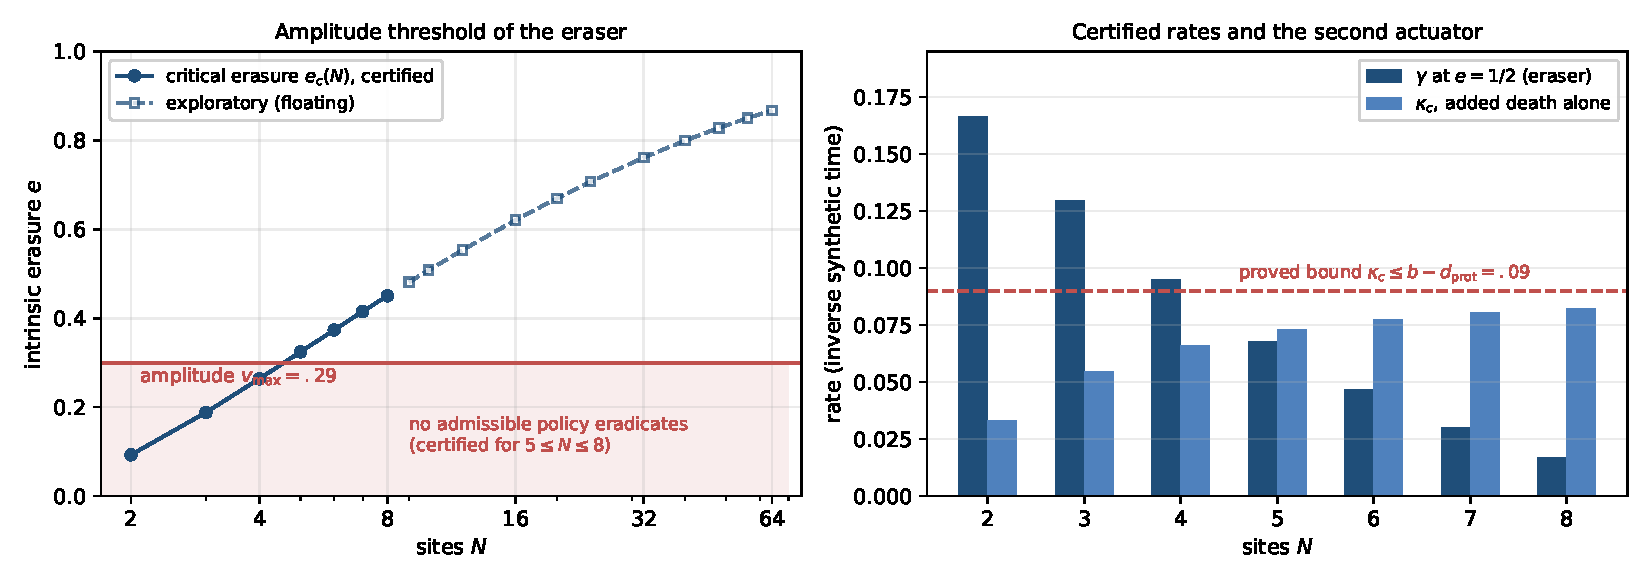
\includegraphics[width=\linewidth]{figures/sites.pdf}
\caption{Left: the eraser's critical intrinsic erasure against memory size.
Filled markers are the exact brackets of Table~\ref{tab:sites}; open markers are
exploratory floating eigenvalue computations for $9\le N\le64$ and are
diagnostics, not certificates. The shaded band is the amplitude used in the
two-site worked example; for $5\le N\le8$ the amplitude floors of
Table~\ref{tab:amp} certify that no policy in that band eradicates. Right:
certified mean contraction rate $\gamma$ of the eraser at the common erasure
$e=1/2$, and the certified threshold $\kappa_c$ of the added-death actuator
acting alone, which Proposition~\ref{prop:kappa} bounds by
$b-d_{\mathrm{prot}}=.09$ for every $N$.}
\label{fig:sites}
\end{figure}

\begin{remark}[Beyond the certified range]\label{rem:bigN}
Floating eigenvalue computations of $\spb(A_e)$, exact in the model but not
rounded rigorously, continue the first column of Table~\ref{tab:sites} as
$e_c\approx.508$ at $N=10$, $.621$ at $N=16$, $.762$ at $N=32$ and $.868$ at
$N=64$. The increments per unit of $\log N$ fall from about $.27$ to about
$.13$ over that range, so the sequence is increasing with decelerating
increments and we do not determine whether $e_c(N)$ remains bounded. What is
proved here is the monotone increase and the factor $4.86$ between $N=2$ and
$N=8$, together with the amplitude floors of Table~\ref{tab:amp}; no assertion
is made uniformly in $N$ for the eraser, and six or eight abstract sites are not
claimed to be a realistic chromatin domain.
\end{remark}

\subsection{The exposure floor barely moves}
\label{sec:expN}

Above the amplitude threshold the picture is different. Table~\ref{tab:expN}
gives, for each $N$, an exact baseline supersolution and the smallest admissible
$c$ for the eraser; the resulting necessary exposure at $n=1$, $\delta=.01$
increases by only $22\%$ between two and eight sites, against the factor $4.86$
in amplitude. Larger inherited state makes the actuator harder to \emph{power},
not appreciably more expensive to \emph{run}, in this source.

\begin{table}[t]
\centering
\caption{Exact baseline exposure certificates for the $N$-site source:
$\PhiB(q)\le0$ and $Rq\le c(1-q)$, with $\eta_{(N,0)}=1-q_{(N,0)}$ and
$B_{\mathrm{nec}}$ evaluated from \eqref{eq:necessary} at $n=1$, $\delta=.01$.
The $N=2$ row is the optimized certificate of Remark~\ref{rem:optcert}, which
supersedes \eqref{eq:q} by $0.54\%$. All vectors are in
the data file \texttt{site\_certificates.json}.}
\label{tab:expN}
\begin{tabular}{rrrr}
\toprule
$N$ & $\eta_{(N,0)}$ & $c$ & $B_{\mathrm{nec}}(1,.01)$\\
\midrule
2 & $.77849912$ & $.916533$ & $4.751365$\\
3 & $.85886565$ & $.884640$ & $5.033717$\\
4 & $.88009489$ & $.857113$ & $5.223867$\\
5 & $.88886370$ & $.832987$ & $5.387069$\\
6 & $.89308829$ & $.811604$ & $5.534843$\\
7 & $.89533756$ & $.792438$ & $5.671883$\\
8 & $.89661409$ & $.775121$ & $5.800437$\\
\bottomrule
\end{tabular}
\end{table}

The constructive side does deteriorate at a fixed amplitude: at the common
admissible erasure $e=1/2$, Table~\ref{tab:sites} gives $\gamma$ falling from
$.166$ to $.017$ and $C$ rising from $3.7$ to $18.6$, so
\eqref{eq:sufficient} yields $B_{\mathrm{suff}}(1,.01)$ growing from $17.4$ at
$N=2$ to $216.8$ at $N=8$. Raising the amplitude helps: a floating optimization
of $v_*/\gamma(v_*)$ over constant actions gives best free-horizon exposures of
about $17.1$ at $N=2$ (at $e=.43$), $27.8$ at $N=4$ (at $e=.74$) and $34.4$ at
$N=6$ (at $e=.91$). These are diagnostics; the certified rows are
Table~\ref{tab:sites}. Either way the eraser's sufficient exposure grows with
$N$ while its necessary exposure does not, so the constant gap widens and the
question of the true optimum becomes harder, not easier, with memory size.

\subsection{A second actuator removes the amplitude obstruction}
\label{sec:combo}

Corollary~\ref{cor:extensions} already admits several additive actuators. The
natural second one here adds death on the protected states,
\begin{equation}\label{eq:kappa}
 \Psi(x)=\kappa\odot(1-x),\qquad
 \kappa_i=\one_{\{a_i>r_i\}},
\end{equation}
with control $u\in[0,u_{\max}]$, so that the death rate in protected states
becomes $d_{\mathrm{prot}}+u$. This is a defined mathematical actuator, not a
claim that a known drug has that selectivity. Because $\kappa\le\one$ we may
take $c_\kappa=1$ in Corollary~\ref{cor:extensions}, so the necessary exposure
for this actuator is exactly $\log\bigl(\eta/(1-(1-\delta)^{1/n})\bigr)$ with
$\eta$ from Table~\ref{tab:expN}.

\begin{proposition}[Dimension-free sufficiency]\label{prop:kappa}
Let a finite-type source have binary division at rate $b$, death rates $d_i$,
count-preserving type changes, and an added-death actuator with nonnegative
indicator vector $\kappa$ as in \eqref{eq:kappa}, held at a constant value
$u=\kappa_*$. If
\[
 \gamma:=\min_i\bigl(d_i+\kappa_*\kappa_i-b\bigr)>0 ,
\]
then $\E|Z_t|\le|z|e^{-\gamma t}$, so $\Prob_z(|Z_t|>0)\le|z|e^{-\gamma t}$ and
extinction is almost sure. In the source \eqref{eq:chem}, where
$b=.1$, $d_{\mathrm{prot}}=.01$ and $d_{\mathrm{unprot}}=.3$, this holds for
every $N$ as soon as $\kappa_*>b-d_{\mathrm{prot}}=.09$, with
$\gamma=\min(\kappa_*-.09,\,.2)$ and $C=1$; hence
\begin{equation}\label{eq:kappasuff}
 B_{\mathrm{suff}}=\frac{\kappa_*}{\min(\kappa_*-.09,\ .2)}\,\log\frac n\delta ,
\end{equation}
minimized at $\kappa_*=.29$, where it equals $1.45\log(n/\delta)$ for every
number of sites.
\end{proposition}

\begin{proof}
Type changes preserve $|z|$ and binary division replaces one cell by two, so
$|Z_t|$ increases by one at rate $b|Z_t|$ and decreases by one at rate
$\sum_iZ_i(t)(d_i+\kappa_*\kappa_i)$. Hence
$\frac{d}{dt}\E|Z_t|=\E\sum_iZ_i(t)(b-d_i-\kappa_*\kappa_i)\le-\gamma\E|Z_t|$,
after the localization of Section~\ref{sec:model}, and Gronwall gives the
bound. Since $|Z_t|$ is integer valued, $\Prob(|Z_t|>0)\le\E|Z_t|$. This is
Proposition~\ref{prop:weight} with $w=\one$, so $C=1$; substituting
$t=\gamma^{-1}\log(n/\delta)$ and $B=\kappa_*t$ gives \eqref{eq:kappasuff}. In
\eqref{eq:chem} the protected states have $b-d=.09$ and the unprotected ones
$b-d=-.2$, giving the stated $\gamma$. Minimizing $\kappa_*/\min(\kappa_*-.09,.2)$
over $\kappa_*>.09$ gives the value $.29/.2=1.45$ at $\kappa_*=.29$.
\end{proof}

\begin{corollary}[Near-sharp exposure constant]\label{cor:sharpconst}
For the actuator \eqref{eq:kappa} in the source \eqref{eq:chem} with amplitude
$u_{\max}\ge.29$, at every $N\le8$,
\[
 \log\frac{\eta_{(N,0)}}{1-(1-\delta)^{1/n}}\ \le\ B^*(n,\delta)
 \ \le\ 1.45\,\log\frac n\delta ,
\]
so $\limsup_{n/\delta\to\infty}B^*(n,\delta)/\log(n/\delta)\le1.45$ while the
liminf is at least $1$. At $n=1$, $\delta=.01$ the certified bracket is
$4.354788\le B^*\le6.677497$, a ratio of $1.533$.
\end{corollary}

\begin{proof}
Combine Corollary~\ref{cor:extensions} with $c_\kappa=1$ and the values of
$\eta$ in Table~\ref{tab:expN} for the lower bound, and
Proposition~\ref{prop:kappa} for the upper. For the liminf use
\eqref{eq:rootbounds}, which gives
$B^*\ge\log(n/\delta)+\log(\eta/2)$.
\end{proof}

This is the sharpness statement that Proposition~\ref{prop:sharp} could not
supply inside a source with genuine inheritance: the exposure floor
\eqref{eq:main} is attained to within a factor $1.45$ by an explicit policy in
the molecular source, uniformly in the size of the inherited state, and the
leading order $\log(n/\delta)$ is exact.

Finally, a small amount of the second actuator repairs the eraser's failure
rather than replacing it. With the eraser held at $e=.3$ --- the amplitude that
Proposition~\ref{prop:ampfloor} certifies cannot eradicate on its own for
$5\le N\le8$ --- the added-death threshold is bracketed exactly at denominator
$10^6$ by
\[
 \kappa_c\in(.008894,.008895),\ (.024937,.024938),\ (.036344,.036345),\
 (.044765,.044766)
\]
for $N=5,6,7,8$ respectively. When the eraser is absent the corresponding
thresholds are
\[
 (.033181,\ .054493,\ .066139,\ .073090,\ .077472,\ .080374,\ .082373)
\]
for $N=2,\dots,8$ --- an increasing sequence that
Proposition~\ref{prop:kappa} caps at $.09$ for every $N$. At six sites an added
death of $.025$ on protected states therefore restores mean contraction where
an eraser amplitude of $.29$ provably cannot.
Additive certificate costs do not by themselves prove or disprove biological
synergy; synergy must be defined against a stated cost, dose pair, endpoint and
admissible policy class, and non-additive target interactions require their own
generator bounds.

\section{Interpretation and an experimental test}
\label{sec:interp}

\subsection{Parameter provenance and observation}

Every numerical rate in Section~\ref{sec:source} is assumed. Basal writing,
feedback, recruited erasure and division allocation specify an inherited-state
mechanism; they are not measured phenotype-switching rates. The
phenotype-to-death map is an explicit functional assumption, and the larger-site
sources of Section~\ref{sec:memory} are further mathematical realizations, not
more accurately calibrated loci. A physical larger domain might use a different
protected-state threshold, enzyme limitation, cooperative recruitment or site
dependence; those would be different sources and should be named as such.

Experiments would need separate division and death event records, calibrated
target engagement, a state observation model and \emph{joint} daughter
observations. Net growth $b-d$ alone is insufficient: the single-type sources
$(b,d)=(.1,.05)$ and $(.2,.15)$ share net growth $.05$ but have eventual
extinction probabilities $1/2$ and $3/4$. A binary reporter has emission rank at
most two and cannot satisfy full-column-rank identification of six arbitrary
states; this blocks that particular identification argument, not the possibility
of identifying a constrained low-dimensional rate family or a
certificate-relevant functional. No numerical range from another cell line or
treatment model is transplanted into this source.

\subsection{Conditional concentration and administered-amount bounds}
\label{sec:pkpd}

Suppose the target-engaging concentration $C(t)\ge0$ has a calibrated
saturating effect
\[
 v(C)=v_{\max}\frac{C}{K+C},\qquad K,v_{\max}>0 .
\]
Here $C$ and $K$ carry concentration units, $v_{\max}$ inverse time, and the
reaction exposure $B_{\mathrm{actual}}=\int_0^Tv(C(t))\,dt$ is dimensionless.
For finite concentration AUC $A=\int_0^TC(t)\,dt$, concavity and Jensen give
\[
 B_{\mathrm{actual}}\le\frac{v_{\max}TA}{KT+A}.
\]
If \eqref{eq:necessary} requires $B_{\mathrm{actual}}\ge B_{\mathrm{req}}>0$,
then
\begin{equation}\label{eq:auc}
 v_{\max}T>B_{\mathrm{req}},\qquad
 A\ge\frac{KTB_{\mathrm{req}}}{v_{\max}T-B_{\mathrm{req}}} .
\end{equation}
The strict inequality holds because finite $A$ makes $A/(KT+A)<1$;
multiplication by positive denominators proves the second. A concentration cap
adds $B_{\mathrm{req}}\le Tv(C_{\max})$.

For $\dot C=I/V_d-kC$ with $C(0)=0$, nonnegative infusion $I$, elimination
$k>0$ and distribution volume $V_d>0$, integration gives
$M=V_d(C(T)+kA)\ge kV_dA$, where $M=\int I$ is the administered amount, so
\begin{equation}\label{eq:mass}
 M\ \ge\ \frac{kV_dKTB_{\mathrm{req}}}{v_{\max}T-B_{\mathrm{req}}} .
\end{equation}
A nonzero initial concentration instead gives $M=V_d(C(T)-C(0)+kA)$ and
subtracts at most $V_dC(0)$ from the lower bound, truncated at zero. These are
necessary conditional bounds, not sufficient regimens; plasma concentration may
not equal the target-engaging concentration; and for a Hill exponent above one
global concavity fails, so one must use a valid concave majorant on the admitted
range rather than reusing this Jensen argument. The inequality prices the eraser
only, not the background killing retained in the example.

The useful content is qualitative and available before calibration: required
engagement close to $v_{\max}T$ forces the necessary AUC to increase sharply.
Section~\ref{sec:memory} sharpens the point. The amplitude floor is a constraint
on $v_{\max}$ alone, and no amount of AUC substitutes for it: if
$v_{\max}<v_c$, \eqref{eq:auc} is not merely hard to satisfy, it is irrelevant,
because Theorem~\ref{thm:amp} rules out eradication at any $A$ and any $T$.

\subsection{A falsifiable low-density comparison}

A prospective microcolony design can compare known founder counts $1,10,100$,
with $AA$-rich and $RR$-rich preparations, equal reaction-exposure early, late
and spread schedules, and separately declared eraser-only and
complete-withdrawal arms. Division and death event tracking should accompany
the molecular readout, with all founders retained in denominators. A fixed-time
viable-cell census and outgrowth over a declared observation window are
different events; undetected cells cannot be equated with extinct lineages
without a validated detection model.

The prediction is a one-sided requirement on exposure, not equality with a
fitted boundary. With a jointly valid parameter and preparation uncertainty
set, the lower bound is minimized and any policy upper bound maximized over the
set before comparing with data. For a simple fixed protocol and independent
replicates, a binomial confidence interval for the correctly observed event can
test that propagated prediction, with multiple-look error controlled in advance.
Survival significantly below a valid lower bound would challenge the adopted
source, actuator law or observation mapping; a data point above the lower bound,
or away from the sufficient upper curve, does not falsify it.

\subsection{Density, space and what the model is not}

The branching model is naturally a low-density persistence or microcolony
model. It is not automatically a model of a macroscopic tumour, and the
large-$n$ statements are mathematical scaling, not a claim that a
million-cell experiment remains density independent. Some extensions reuse the
barrier directly: for a population-dependent source it suffices to prove the
analogue of \eqref{eq:barrier} uniformly over the admitted population states and
environments, and a constructive upper bound survives if the weighted drift
remains uniformly negative. Reducing division is not automatically favourable
here, because division also redistributes marks and the sign of
$D_i(x,x)-x_i$ need not be uniform; density-dependent birth suppression
therefore cannot be inserted by an unsupported monotonicity argument. Spatial
migration or hidden carriers require explicit additional state variables and
generator terms, and persistent immigration destroys the absorbing-zero setup
entirely.

\section{Discussion}
\label{sec:disc}

The remaining-exposure construction establishes a population-dependent floor
against arbitrary admitted feedback. The product in that floor is a function of
the whole configuration, not an independence approximation during treatment, and
its founder dependence survives the coupling that a common controller
introduces. The amplitude construction is a different certificate with a
different conclusion: below a critical actuator strength the survival floor does
not decay at all, so no budget and no schedule can help. Separating the two is
what makes the memory-size question well posed, and what turns a diagnostic
about one constant action into a statement about every policy.

Three concrete conclusions follow for the molecular source. First, the
obstruction that scales badly with the size of the inherited state is
\emph{amplitude}, not exposure: between two and eight sites the certified
critical erasure rises by a factor $4.86$ while the necessary exposure rises by
$22\%$. Second, the amplitude used in the two-site worked example provably fails
at five to eight sites, against every predictable feedback policy, at infinite
budget and infinite time. Third, the failure is a property of that actuator:
added death on protected states has a threshold bounded by $b-d_{\mathrm{prot}}$
for every $N$ by an elementary total-count argument, delivers a dimension-free
sufficient exposure $1.45\log(n/\delta)$, and attains the exposure floor to
within a factor $1.533$ at $n=1$, $\delta=.01$. That last point also supplies
the sharpness that Proposition~\ref{prop:sharp} could only give in a degenerate
comparison source.

What remains open is quantitative and specific. For the eraser at two sites the
certified bracket at $T=100$ is $4.7257\le B^*\le11.6$, and
Remark~\ref{rem:optcert} shows the lower endpoint is within $0.54\%$ of what
certificate optimization alone can deliver, so the residual factor of about
$2.45$ is not a defect of the chosen supersolution. Closing it requires either a
richer population barrier or a better policy, and the natural next experiment is
to certify a small phase family selected by backward sensitivity of the
generating-function flow and compare it with a population-budget barrier that
does not factor through a single vector $q$. Whether $e_c(N)$ remains bounded as
$N\to\infty$ is open; the exploratory evidence of Remark~\ref{rem:bigN} is
consistent with either answer, and a proof in either direction would say
something structural about how fast inherited memory can be defeated by a
single reaction-rate actuator.

Uniform constants in site count for the eraser, density-dependent populations,
empirical target engagement, a global solution of the associated dynamic
programming equation, and full stochastic formalization all remain outside this
paper. They are explicit future scopes and not hidden assumptions: the
formalization boundary is stated in Appendix~\ref{app:boundary}, the evidence
type of every displayed quantity is labelled, and the exact vectors behind every
certificate are released with the source package.


\appendix
\section{Validated generating-function calculation}
\label{app:validated}

This appendix specifies the proof behind \eqref{eq:validated} independently of
any floating ODE solver. For constant erasure write $\Phi(z)=Jz+d+.1D(z,z)$
with $J=Q-\diag(d+.1)$. Taylor coefficients at any initial point obey
\begin{equation}\label{eq:recurrence}
 c_0=z,\qquad
 c_{k+1}=\frac1{k+1}\left[Jc_k+\one_{\{k=0\}}d
              +.1\sum_{j=0}^kD(c_j,c_{k-j})\right].
\end{equation}
The unit cube is invariant: at $z_i=0$ every inward term is nonnegative, and at
$z_i=1$ the switching, death and offspring terms sum to a nonpositive value. On
the cube the Jacobian is Metzler, with row sums
$-d_i+.1\bigl(\sum_j\partial_jD_i(z,z)-1\bigr)\le.1-d_i\le.09$. The upper right
derivative of the sup norm of a difference of solutions is therefore at most
$.09$ times that norm, by the mean-value Jacobian and the maximal-coordinate
argument, so the flow is $e^{.09t}$-Lipschitz in that norm. This is a one-sided
logarithmic-norm bound \citep{soderlind2006}, not a bound on the norm of the
Jacobian itself.

All interval endpoints in \texttt{scripts/validated\_pgf.py} are integers
divided by $2^{110}$. Addition and subtraction are exact at that scale.
Multiplication takes the smallest and largest of the four integer products and
rounds outwards after division by $2^{110}$; division by a positive integer also
rounds outwards; rational inputs are enclosed by floor and ceiling. Induction on
\eqref{eq:recurrence} proves inclusion of each exact coefficient
\citep{moore2009}.

Use steps $h=1/20$ and a degree-$11$ Taylor polynomial. First evaluate the
recurrence to $c_{12}$ with $c_0=[0,1]^6$ and let $M$ be the largest absolute
endpoint; at every point of the exact trajectory
$\|z^{(12)}\|_\infty/12!\le M$, so Taylor's integral remainder on a step is
bounded by $Mh^{12}$. The bounds used are approximately $4.828\cdot10^{-6}$ for
$e=.01$ and $1.806\cdot10^{-4}$ for $e=.3$; the exact fractions are in
the data file \texttt{validated\_policy.json}.

For each step, compute the polynomial at the dyadic centre using outward
interval operations, add the remainder, and choose a dyadic midpoint projected
onto the unit cube. The maximum distance from that centre to the interval, plus
the remainder, bounds the local error; this local enclosure is defined once and
its radius enters the error recurrence once. If $E$ bounds the incoming sup-norm
error, propagate it as
\[
 E_{\mathrm{new}}\ \le\ \frac{E}{1-.09h}+E_{\mathrm{local}},
\]
rounded upward, which is valid because $e^{.09h}\le(1-.09h)^{-1}$ for
$.09h<1$. Projection does not invalidate the calculation: the local distance is
computed after projection and the exact flow remains in the cube. Starting at
zero, $1200$ low-erasure steps followed by $800$ high-erasure steps give total
error
\[
 E=\frac{3241002892060825847}{1298074214633706907132624082305024}
 \ <\ 2.497\cdot10^{-15}.
\]
The enclosure accounts separately for coefficient rounding, polynomial
evaluation, local truncation, error propagation and phase composition. It is an
exact-arithmetic computation together with the preceding conventional enclosure
proof \citep{nedialkov1999}, not a formalization of the numerical algorithm in a
proof assistant. No unproved floating tolerance enters the certificate.

\section{The preparation counterexample}
\label{app:taylor}

For $u(0)=0$ the first Taylor coefficients of the backward flow are $c_1=d$,
$c_2=J_ed/2$, $c_3=(J_ec_2+.1D(d,d))/3$ and $c_4=(J_ec_3+.2D(d,c_2))/4$.
Substituting in the $RR$ coordinate of the two-site source gives
\[
 (c_4)_{RR}=-\frac{16087}{8000000}-\frac{29}{480000}\,e
            -\frac{29}{40000}\,e^2 .
\]
The coefficients through order three agree between $e=.01$ and $e=.3$, and
their fourth-order difference is the coefficient displayed in
\eqref{eq:taylor}:
\[
 (c_4)_{RR}\big|_{e=.3}-(c_4)_{RR}\big|_{e=.01}
 =-\frac{49619}{600000000}.
\]
Analyticity of a polynomial ODE near zero then proves the strict sign on some
positive interval, which is the content of \eqref{eq:taylor}. Numerically, at
$t=1$ the two extinction probabilities are $.2493000462$ and $.2492590475$, a
difference of about $4.1\cdot10^{-5}$; these displayed finite-time values are
diagnostics and not part of the analytic proof. The example shows that stronger
erasure can lower the extinction probability at short times from a
repressed preparation, because erasure also removes repressive marks and
permits access to the protected active states of this source. It is a
counterexample to universal monotonicity in the actuator, which is one reason
the amplitude certificate of Theorem~\ref{thm:amp} is stated against arbitrary
predictable policies rather than against constant actions.

\section{\texorpdfstring{Certificates for the $N$-site source}%
                        {Certificates for the N-site source}}
\label{app:certs}

This appendix states how the certificates of Section~\ref{sec:memory} were
produced and verified, and displays the one that carries the paper's negative
conclusion. All vectors, all slacks and the reconstruction of the source
matrices are in the data file \texttt{site\_certificates.json}; the source
module is \texttt{site\_source.py}, the driver that produces the certificates
is \texttt{make\_certificates.py}, and \texttt{verify\_certificates.py} replays
every check listed below. Every displayed inequality is checked
with \texttt{fractions.Fraction} arithmetic against a source matrix
reconstructed from \eqref{eq:chem}, the binomial allocation law and the death
rule, never against stored matrix entries. Floating computation is used only to
propose candidate vectors.

\subsection{Reconstruction and state order}

States are generated as $(a,r)$ with $a$ increasing outermost and $r$
increasing innermost, subject to $a+r\le N$, which reproduces
$(UU,UR,RR,AU,AR,AA)$ at $N=2$. The chemical generator uses \eqref{eq:chem}
with rational $e$; the single-daughter marginal is
$\Lambda_{(a,r),(a',r')}=2^{-(a+r)}\binom a{a'}\binom r{r'}$; the first-moment
matrix is \eqref{eq:meanmatrix} with $L=2\Lambda$; and the joint daughter law
pairs $(a',r')$ with $(a-a',r-r')$ at the same probability, so sibling
correlation is retained in $\Phi$ and only the mean operator uses $\Lambda$.

\subsection{Three kinds of certificate}

\paragraph{Spectral sign (Table~\ref{tab:sites}, first column).}
For each rational $e$ the matrix $M=-A_e$ is a $Z$-matrix, and all its leading
principal minors are computed by exact elimination. By \eqref{eq:mtest} their
positivity is equivalent to $\spb(A_e)<0$. Bisection on $e$ at denominator
$10^6$ gives the brackets; the sign at each endpoint is additionally confirmed
by a positive rational vector and \eqref{eq:cw}. At $e=3/10$ the resulting
two-sided brackets are
\[
 \spb(A_{.3})\in\Bigl[-\tfrac7{500},-\tfrac{139}{10000}\Bigr]\ (N=4),
 \qquad
 \spb(A_{.3})\in\Bigl[\tfrac{239}{10000},\tfrac3{125}\Bigr]\ (N=6),
\]
with the $15$- and $28$-dimensional witnesses recorded in the data file.

\paragraph{Contraction weights (Table~\ref{tab:sites}, last two columns).}
The Perron vector of $A_{1/2}$ is computed in floating arithmetic, rounded to a
positive rational vector $w$, and the inequalities $A_{1/2}w\le-\gamma w$ are
then verified exactly for a rational $\gamma$ rounded down from
$\min_i(-(A_{1/2}w)_i/w_i)$. Only the verified inequality is used;
no eigenvalue rounded to a favourable sign enters a proof.

\paragraph{Amplitude floors (Table~\ref{tab:amp}).}
The required object is a single $q$ with $\PhiB(q)\le0$ and
$\Phi_{v_{\max}}(q)\le0$. The minimal such $q$ is the least fixed point of the
componentwise maximum
\[
 \mathcal M(q)_i=\max\bigl\{\PhiB(q)_i,\ \Phi_{v_{\max}}(q)_i\bigr\},
\]
which is reached by monotone iteration from $0$ and polished by Newton's method
on the active selection. Rounding that fixed point is delicate because the
inequalities are tight there, so instead of rounding we retract along the
segment of Lemma~\ref{lem:segment}: with $h=1-q$ and $a=99/100$, the vector
$1-ah$ satisfies
\[
 \Phi_v(1-ah)\le a\Phi_v(q)-a(1-a)\,b\odot D(h,h)\le-\tfrac{99}{10000}\,b\odot D(h,h)<0
\]
for every admitted $v$, with a strictly positive margin that dominates the
rounding perturbation. The retracted vector is then written with denominator
$10^8$ (or $10^{10}$ where the margin is smaller) and both inequality systems
are verified exactly. The cost is a $1\%$ reduction of $\eta$, which is included
in every value reported in Table~\ref{tab:amp}.

\subsection{The six-site amplitude floor}

At $N=6$ with baseline $e=.01$ and eraser amplitude $v_{\max}=.29$, the vector
$q=10^{-8}\cdot Q$ with
\[
\begin{array}{r@{\;}l}
Q=(&94286500,\ 98272968,\ 99056686,\ 99331683,\ 99457438,\ 99525067,\ 99565657,\\
   &70705469,\ 86090037,\ 93106756,\ 96203017,\ 97651735,\ 98389280,\\
   &61949773,\ 75113027,\ 85816369,\ 91719992,\ 94863984,\\
   &58024251,\ 68295718,\ 77595263,\ 86256272,\\
   &55984798,\ 63905275,\ 71672698,\\
   &54795331,\ 60968199,\\
   &54037279\,)
\end{array}
\]
in the state order $(0,0),(0,1),\dots,(0,6),(1,0),\dots,(1,5),\dots,(6,0)$
satisfies $\Phi_{.01}(q)\le0$ and $\Phi_{.3}(q)\le0$ in exact rational
arithmetic, with largest coordinate slacks $-6.47\cdot10^{-8}$ and
$-3.30\cdot10^{-6}$ respectively. By Theorem~\ref{thm:amp}, every predictable
policy with eraser amplitude at most $.29$ --- including cell-specific policies,
at unbounded budget and unbounded horizon --- leaves the six-site population
alive with probability at least $1-(1-\eta)^n$ from $n$ founders of type
$(6,0)$, where $\eta=1-54037279/10^8=.45962721$.

\subsection{Reproduction}

The single command \texttt{python verify\_certificates.py} replays every exact
check reported in Section~\ref{sec:memory}: it reconstructs the source at each
$N$, re-verifies the $M$-matrix brackets, the Collatz--Wielandt witnesses, the
contraction weights, the baseline exposure certificates, the amplitude floors
and the added-death thresholds, and prints each verdict. The two-site checks of
Section~\ref{sec:source} and the enclosure \eqref{eq:validated} are replayed by
the scripts inherited from the two-site study. No floating optimizer and no
Monte Carlo simulation is needed to check any claim; floating computation
appears only in the candidate search and in the clearly labelled diagnostics of
Remark~\ref{rem:bigN} and Figure~\ref{fig:policy}.

\input{sections/app_boundary}

\begingroup
\small
\setlength{\bibsep}{3pt}
\bibliographystyle{plainnat}
\bibliography{references}
\endgroup
\end{document}
